\chapter{异常}

\section{异常}

\subsection{异常(Exception)}

异常就是程序在运行过程中出现的非正常的情况。异常本身是一个类,产生异常就是创建异常对象并抛出一个异常对象。Java处理异常的方法是中断处理。\\

如果程序遇到了未经处理的异常,会导致这个程序无法进行编译或者运行。\\

Throwable类用来描述所有的不正常的情况。Throwable有两个子类:

\begin{enumerate}
    \item Error:描述发生在JVM虚拟机级别的错误信息,这些错误无法被处理。
    \item Exception:描述程序遇到的异常,异常是可以被捕获处理的。
\end{enumerate}

\begin{figure}[H]
    \centering
    \begin{forest}
        for tree={% style of tree nodes
        draw, semithick, rounded corners, drop shadow,
        top color = red!20,
        bottom color = red!40,
        text width = 47mm, text badly centered,
        edge = {draw, semithick},
        parent anchor = east,
        child anchor = west,
        grow = east,
        s sep = 5mm,    % sibling distance
        l sep = 4mm,    % level distance
        }
        [Exception
            [RuntimeException
                    [UnknownTypeException]
                    [ArrayIndexOutOfBounds Exception]
                    [IllegalArgumentException]
                    [NullPointerException]
                    [ClassNotFoundException]
                    [MissingResourceException]
                    [ArithmeticException]
            ]
            %
            [IOException
                    [FileNotFoundException]
                    [EOFException]
            ]
        ]
    \end{forest}
    \caption{异常分类}
\end{figure}

\mybox{数组越界异常}

\begin{lstlisting}[language=Java]
public class ArrayIndexException {
    public static void main(String[] args) {
        int[] arr = {0, 1, 2, 3, 4};
        System.out.println(arr[5]);
    }
}
\end{lstlisting}

\begin{tcolorbox}
    \mybox{运行结果}
    \begin{verbatim}
Exception in thread "main"
java.lang.ArrayIndexOutOfBoundsException:
    Index 5 out of bounds for length 5
	\end{verbatim}
\end{tcolorbox}

普通的异常会导致程序无法完成编译,这样的异常被称为非运行时异常(non-runtime exception),但是由于异常是发生在编译时期的,因此常常称为编译时异常。\\

Exception类有一个子类RuntimeException类对异常进了自动的处理,这种异常不会影响程序的编译,但是在运行中如果遇到了这种异常,会导致程序执行的强制停止。这样的异常被称为运行时异常。

\newpage

\section{异常的捕获处理}

\subsection{try-catch}

如果一个异常不去处理,会导致程序无法编译或者运行。使用try-catch语句可以捕获并处理异常。

\vspace{-0.5cm}

\begin{lstlisting}[language=Java]
try {
    // 可能出现异常的代码
} catch(exceptionType e) {
    // 异常的类型和catch的异常的类型匹配,执行此处逻辑
}
\end{lstlisting}

一个异常如果被捕获处理了,那么将不再影响程序的执行。

\begin{figure}[H]
    \centering
    
\includegraphics{img/Chapter8/8-2/1.png}
\end{figure}

如果在try结构中出现了异常,那么从异常出现的位置开始,try结构中往后的代码将不再执行。\\

\mybox{捕获数组越界异常}

\begin{lstlisting}[language=Java]
public class TryCatch {
    public static void main(String[] args) {
        int[] arr = {0, 1, 2, 3, 4};
        try {
            int elem = arr[5];
            System.out.println("elem = " + elem);
        } catch(ArrayIndexOutOfBoundsException e) {
            System.out.println("数组下标越界异常被捕获处理了");
        }
    }
}
\end{lstlisting}

\begin{tcolorbox}
    \mybox{运行结果}
    \begin{verbatim}
数组下标越界异常被捕获处理了
	\end{verbatim}
\end{tcolorbox}

\vspace{0.5cm}

\subsection{finally}

finally出现在try-catch结构的结尾,无论try代码段中有没有异常、无论try里面出现的异常有没有被捕获处理,finally中的代码始终会执行。基于这个特点,常常在finally中进行资源释放、流的关闭等操作。\\

\mybox{finally}

\begin{lstlisting}[language=Java]
import java.util.Scanner;

public class Finally {
    public static void main(String[] args) {
        Scanner scanner = new Scanner(System.in);
        int[] arr = {0, 1, 2, 3, 4};
        try {
            System.out.print("输入新数据:");
            arr[5] = scanner.nextInt();
        } catch(ArrayIndexOutOfBoundsException e) {
            System.out.println("数组下标越界异常被捕获处理了");
        } finally {
            System.out.println("关闭输入流...");
            scanner.close();
        }
    }
}
\end{lstlisting}

\begin{tcolorbox}
    \mybox{运行结果}
    \begin{verbatim}
输入新数据:5
数组下标越界异常被捕获处理了
关闭输入流...
	\end{verbatim}
\end{tcolorbox}

\vspace{0.5cm}

\subsection{catch}

如果多个catch捕获的异常类型之间没有继承关系存在,此时先后顺序无所谓。\\

如果多个catch捕获的异常类型之间存在继承关系,则必须保证父类异常在后,子类异常在前。\\

\mybox{catch}

\begin{lstlisting}[language=Java]
import java.util.Scanner;
import java.util.InputMismatchException;

public class Catch {
    public static void main(String[] args) {
        Scanner scanner = new Scanner(System.in);
        try {
            System.out.println("【除法运算】");
            System.out.print("输入被除数:");
            int num1 = scanner.nextInt();
            System.out.print("输入除数:");
            int num2 = scanner.nextInt();
            int result = num1 / num2;
            System.out.println("结果:" + result);
        } catch(ArithmeticException e) {
            System.err.println("算术异常");
        } catch(InputMismatchException e) {
            System.err.println("输入类型异常");
        } finally {
            scanner.close();
        }
    }
}
\end{lstlisting}

\begin{tcolorbox}
    \mybox{运行结果}
    \begin{verbatim}
【除法运算】
输入被除数:10
输入除数:0
算术异常
	\end{verbatim}

    \mybox{运行结果}
    \begin{verbatim}
【除法运算】
输入被除数:hey
输入类型异常
	\end{verbatim}
\end{tcolorbox}

\newpage

\section{throw与throws}

\subsection{throw / throws}

throw关键字用于抛出一个异常,一般用于程序出现某种逻辑时程序员主动抛出某种特定类型的异常。

\vspace{-0.5cm}

\begin{lstlisting}[language=Java]
throw e;
\end{lstlisting}

throws关键字用在声明方法的时候,表示该方法可能要抛出异常。定义了throws异常抛出类型的方法,在当前的方法中可以不处理这个异常,由调用方处理。

\vspace{-0.5cm}

\begin{lstlisting}[language=Java]
accessModifier returnType func([paramList]) throws exceptionType {
    // code
}
\end{lstlisting}

\begin{figure}[H]
    \centering
    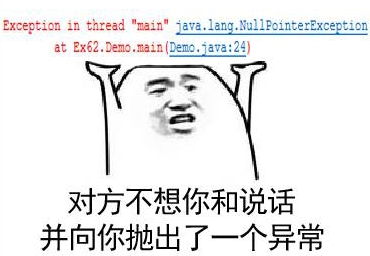
\includegraphics{img/Chapter8/8-3/1.png}
\end{figure}

\mybox{抛出异常}

\begin{lstlisting}[language=Java]
public class Person {
    private int age;
    
    public void setAge(int age) throws Exception {
        if(age < 0 || age > 130) {
            throw new Exception();
        }
        this.age = age; 
    }
    
    public static void main(String[] args) {
        try {
            Person person = new Person();
            person.setAge(-1);
        } catch(Exception e) {
            System.out.println("年龄异常");
        }
    }
}
\end{lstlisting}

\begin{tcolorbox}
    \mybox{运行结果}
    \begin{verbatim}
年龄异常
	\end{verbatim}
\end{tcolorbox}

\newpage

\section{自定义异常}

\subsection{自定义异常}

使用异常是为了处理一些重大的逻辑bug,这些逻辑bug可能会导致程序的崩溃。此时,可以使用异常机制,强迫修改这个bug。\\

系统中提供了很多的异常类型,但是异常类型提供地再多,也无法满足所有的需求。当需要的异常类型系统没有提供的时候,此时就需要自定义异常了。\\

系统提供的每一种异常都是一个类,所以自定义异常其实就是写一个自定义的异常类。自定义的异常类,理论上来讲,类名可以任意定义,但是出于规范,一般都会以Exception作为结尾,例如ArrayIndexOutOfBoundsException、NullPointerException、ArithmeticException等。\\

如果要自定义一个编译时异常,需要继承自Exception类,如果要自定义一个运行时异常,需要继承自RuntimeException类。\\

\mybox{自定义异常}

\begin{lstlisting}[language=Java, title=AgeException.java]
public class AgeException extends RuntimeException {
    public AgeException() {
        super("年龄异常");
    }
    
    public AgeException(int age) {
        super("年龄异常:" + age);
    }
}
\end{lstlisting}

\begin{lstlisting}[language=Java, title=Person.java]
public class Person {
    private int age;
    
    public void setAge(int age) throws AgeException {
        if(age < 0 || age > 130) {
            throw new AgeException(age);
        }
        this.age = age;
    }
    
    public static void main(String[] args) {
        try {
            Person person = new Person();
            person.setAge(-1);
        } catch(AgeException e) {
            e.printStackTrace();
        }
    }
}
\end{lstlisting}

\begin{tcolorbox}
    \mybox{运行结果}
    \begin{verbatim}
AgeException: 年龄异常:-1
at Person.setAge(Person.java:6)
at Person.main(Person.java:15)
	\end{verbatim}
\end{tcolorbox}

\newpage